\begin{figure}[ht!]
    \centering
    % \begin{tabular}[c]{ccc}
    % \begin{subfigure}[c]{0.31\textwidth}
    %     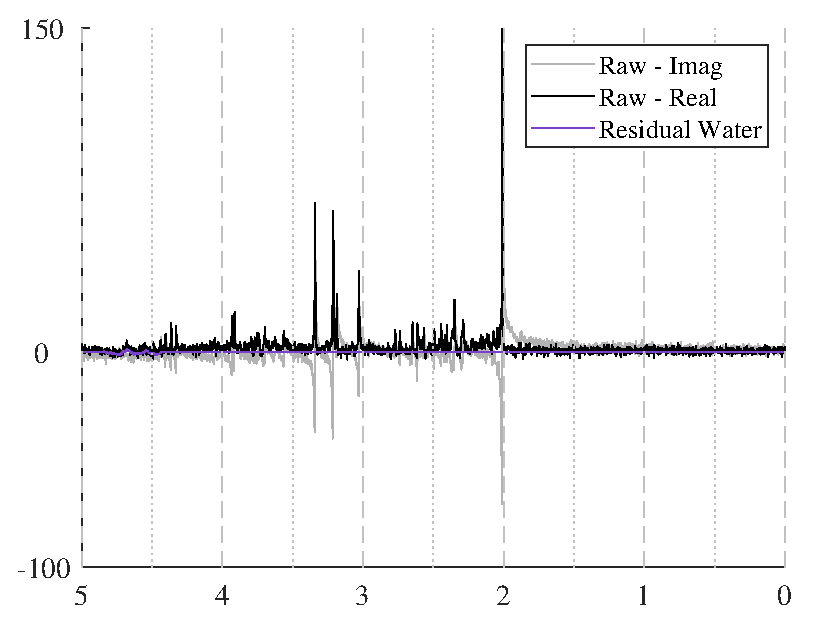
\includegraphics[width=0.93\textwidth]{images/samples_by_artifact/30ms_artifact_samples_gaussian_1.eps}
    %     \caption{Gaussian = 1.0 Hz}
    %     \vspace{3pt}
    % \end{subfigure}&
    % \begin{subfigure}[c]{0.31\textwidth}
    %     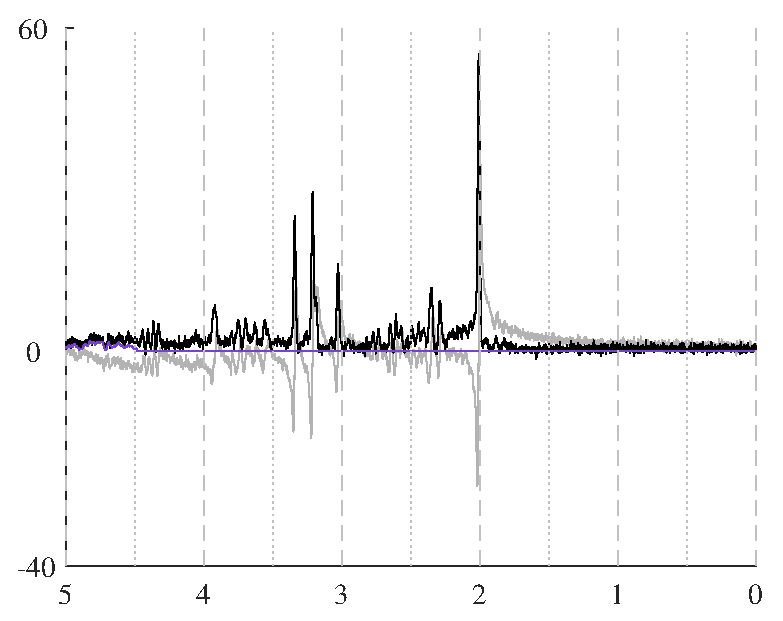
\includegraphics[width=0.93\textwidth]{images/samples_by_artifact/30ms_artifact_samples_gaussian_2.eps}
    %     \caption{Gaussian = 14.9 Hz}
    %     \vspace{3pt}
    % \end{subfigure}&
    % \begin{subfigure}[c]{0.31\textwidth}
    %     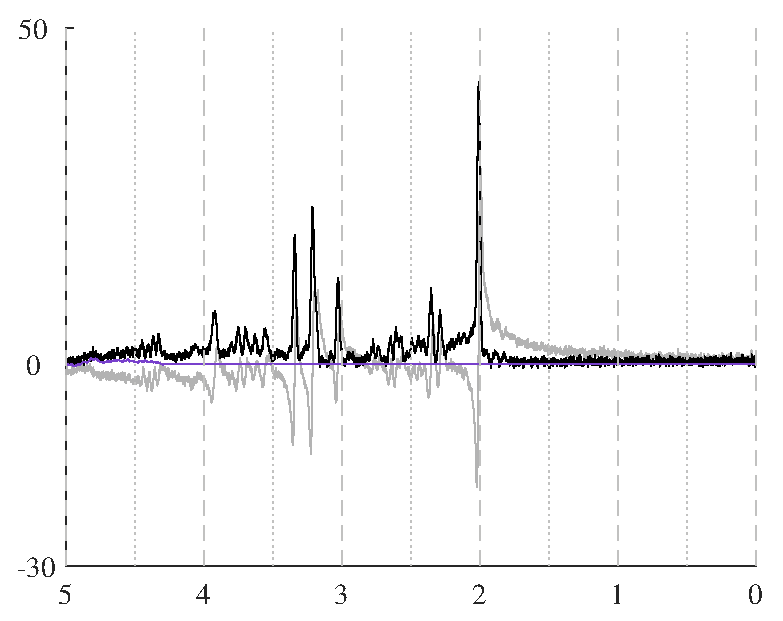
\includegraphics[width=0.93\textwidth]{images/samples_by_artifact/30ms_artifact_samples_gaussian_3.eps}
    %     \caption{Gaussian = 28.8 Hz}
    %     \vspace{3pt}
    % \end{subfigure}\\
    % \begin{subfigure}[c]{0.31\textwidth}
    %     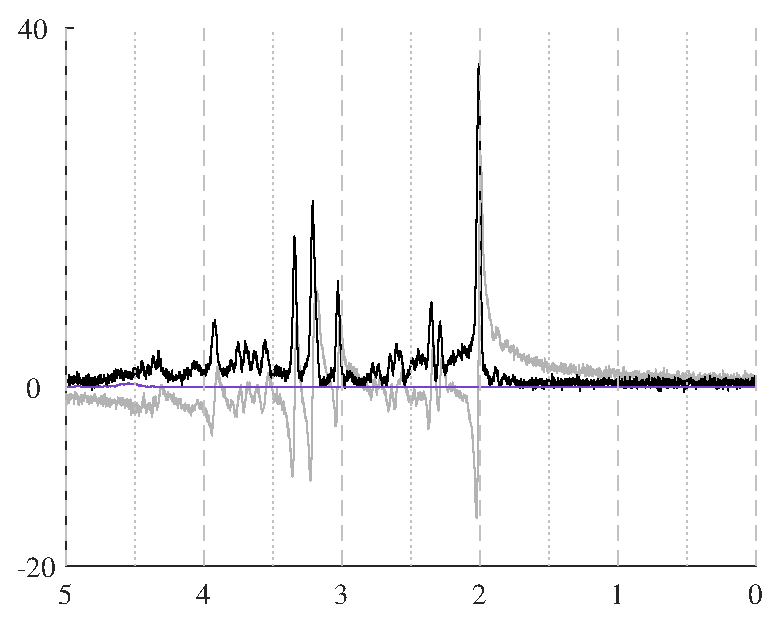
\includegraphics[width=0.93\textwidth]{images/samples_by_artifact/30ms_artifact_samples_gaussian_4.eps}
    %     \caption{Gaussian = 42.8 Hz}
    %     \vspace{3pt}
    % \end{subfigure}&
    % \begin{subfigure}[c]{0.31\textwidth}
    %     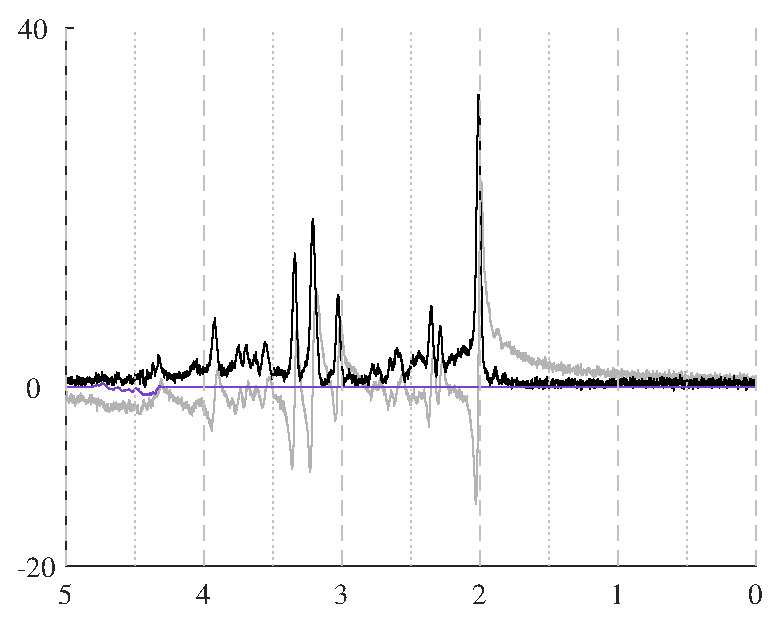
\includegraphics[width=0.93\textwidth]{images/samples_by_artifact/30ms_artifact_samples_gaussian_5.eps}
    %     \caption{Gaussian = 56.7 Hz}
    %     \vspace{3pt}
    % \end{subfigure}&%
    % \begin{subfigure}[c]{0.31\textwidth}
    %     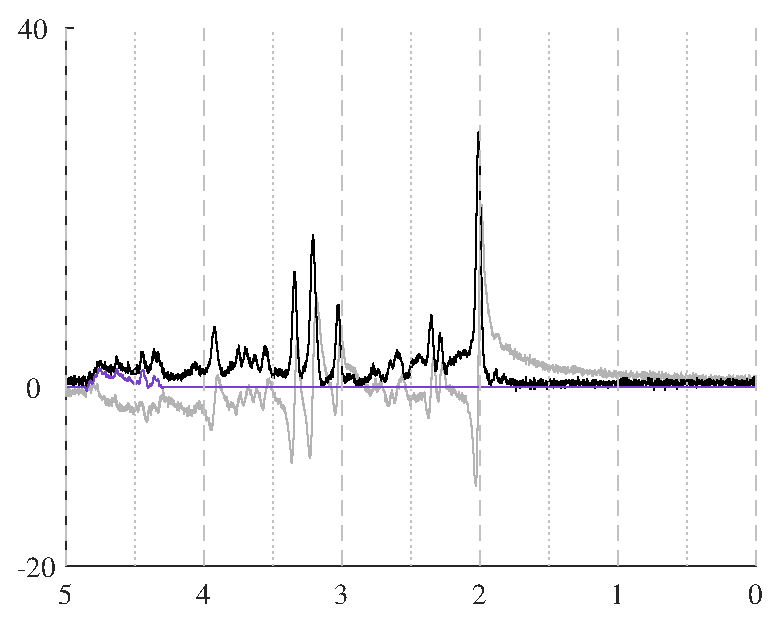
\includegraphics[width=0.93\textwidth]{images/samples_by_artifact/30ms_artifact_samples_gaussian_6.eps}
    %     \caption{Gaussian = 70.7 Hz}
    %     \vspace{3pt}
    % \end{subfigure}\\
    % \end{tabular}
    \includegraphics[width=\textwidth,keepaspectratio]{images/compiled_figures/MRS_Sim_Figure_9_Gaussian_Broadening_samples.png}
    \caption{Gaussian broadening values were sampled from [0,70.17] in increasing order, as displayed beneath each plot. The lorentzian broadening was left unscaled (scaling coeffient = 1.0 corresponding to Fig. \ref{fig:30ms samples lorentzians}). The spectral SNR = 15 and phase offsets and eddy currents were omitted.}
    \label{fig:30ms samples gaussians}
\end{figure}

